
%% bare_conf_compsoc.tex
%% V1.4b
%% 2015/08/26
%% by Michael Shell
%% See:
%% http://www.michaelshell.org/
%% for current contact information.
%%
%% This is a skeleton file demonstrating the use of IEEEtran.cls
%% (requires IEEEtran.cls version 1.8b or later) with an IEEE Computer
%% Society conference paper.
%%
%% Support sites:
%% http://www.michaelshell.org/tex/ieeetran/
%% http://www.ctan.org/pkg/ieeetran
%% and
%% http://www.ieee.org/

%%*************************************************************************
%% Legal Notice:
%% This code is offered as-is without any warranty either expressed or
%% implied; without even the implied warranty of MERCHANTABILITY or
%% FITNESS FOR A PARTICULAR PURPOSE! 
%% User assumes all risk.
%% In no event shall the IEEE or any contributor to this code be liable for
%% any damages or losses, including, but not limited to, incidental,
%% consequential, or any other damages, resulting from the use or misuse
%% of any information contained here.
%%
%% All comments are the opinions of their respective authors and are not
%% necessarily endorsed by the IEEE.
%%
%% This work is distributed under the LaTeX Project Public License (LPPL)
%% ( http://www.latex-project.org/ ) version 1.3, and may be freely used,
%% distributed and modified. A copy of the LPPL, version 1.3, is included
%% in the base LaTeX documentation of all distributions of LaTeX released
%% 2003/12/01 or later.
%% Retain all contribution notices and credits.
%% ** Modified files should be clearly indicated as such, including  **
%% ** renaming them and changing author support contact information. **
%%*************************************************************************


% *** Authors should verify (and, if needed, correct) their LaTeX system  ***
% *** with the testflow diagnostic prior to trusting their LaTeX platform ***
% *** with production work. The IEEE's font choices and paper sizes can   ***
% *** trigger bugs that do not appear when using other class files.       ***                          ***
% The testflow support page is at:
% http://www.michaelshell.org/tex/testflow/



\documentclass[conference,compsoc]{IEEEtran}
  % \usepackage{graphicx}
  % \usepackage{caption}
  % \usepackage{booktabs}
  \usepackage{tabularx}
    % Some/most Computer Society conferences require the compsoc mode option,
    % but others may want the standard conference format.
    %
    % If IEEEtran.cls has not been installed into the LaTeX system files,
    % manually specify the path to it like:
    % \documentclass[conference,compsoc]{../sty/IEEEtran}
    
    
    
    
    
    % Some very useful LaTeX packages include:
    % (uncomment the ones you want to load)
    
    
    % *** MISC UTILITY PACKAGES ***
    %
    %\usepackage{ifpdf}
    % Heiko Oberdiek's ifpdf.sty is very useful if you need conditional
    % compilation based on whether the output is pdf or dvi.
    % usage:
    % \ifpdf
    %   % pdf code
    % \else
    %   % dvi code
    % \fi
    % The latest version of ifpdf.sty can be obtained from:
    % http://www.ctan.org/pkg/ifpdf
    % Also, note that IEEEtran.cls V1.7 and later provides a builtin
    % \ifCLASSINFOpdf conditional that works the same way.
    % When switching from latex to pdflatex and vice-versa, the compiler may
    % have to be run twice to clear warning/error messages.
    
    
    
    
    
    
    % *** CITATION PACKAGES ***
    %
    \ifCLASSOPTIONcompsoc
      % IEEE Computer Society needs nocompress option
      % requires cite.sty v4.0 or later (November 2003)
      \usepackage[nocompress]{cite}
    \else
      % normal IEEE
      \usepackage{cite}
    \fi
    % cite.sty was written by Donald Arseneau
    % V1.6 and later of IEEEtran pre-defines the format of the cite.sty package
    % \cite{} output to follow that of the IEEE. Loading the cite package will
    % result in citation numbers being automatically sorted and properly
    % "compressed/ranged". e.g., [1], [9], [2], [7], [5], [6] without using
    % cite.sty will become [1], [2], [5]--[7], [9] using cite.sty. cite.sty's
    % \cite will automatically add leading space, if needed. Use cite.sty's
    % noadjust option (cite.sty V3.8 and later) if you want to turn this off
    % such as if a citation ever needs to be enclosed in parenthesis.
    % cite.sty is already installed on most LaTeX systems. Be sure and use
    % version 5.0 (2009-03-20) and later if using hyperref.sty.
    % The latest version can be obtained at:
    % http://www.ctan.org/pkg/cite
    % The documentation is contained in the cite.sty file itself.
    %
    % Note that some packages require special options to format as the Computer
    % Society requires. In particular, Computer Society  papers do not use
    % compressed citation ranges as is done in typical IEEE papers
    % (e.g., [1]-[4]). Instead, they list every citation separately in order
    % (e.g., [1], [2], [3], [4]). To get the latter we need to load the cite
    % package with the nocompress option which is supported by cite.sty v4.0
    % and later.
    
    
    
    
    
    % *** GRAPHICS RELATED PACKAGES ***
    %
    \ifCLASSINFOpdf
      \usepackage[pdftex]{graphicx}
      % declare the path(s) where your graphic files are
      \graphicspath{{../}}
      % and their extensions so you won't have to specify these with
      % every instance of \includegraphics
  %     \DeclareGraphicsExtensions{.pdf,.jpeg,.png}
    \else
      % or other class option (dvipsone, dvipdf, if not using dvips). graphicx
      % will default to the driver specified in the system graphics.cfg if no
      % driver is specified.
      % \usepackage[dvips]{graphicx}
      % declare the path(s) where your graphic files are
      % \graphicspath{{../eps/}}
      % and their extensions so you won't have to specify these with
      % every instance of \includegraphics
      % \DeclareGraphicsExtensions{.eps}
    \fi
    % graphicx was written by David Carlisle and Sebastian Rahtz. It is
    % required if you want graphics, photos, etc. graphicx.sty is already
    % installed on most LaTeX systems. The latest version and documentation
    % can be obtained at: 
    % http://www.ctan.org/pkg/graphicx
    % Another good source of documentation is "Using Imported Graphics in
    % LaTeX2e" by Keith Reckdahl which can be found at:
    % http://www.ctan.org/pkg/epslatex
    %
    % latex, and pdflatex in dvi mode, support graphics in encapsulated
    % postscript (.eps) format. pdflatex in pdf mode supports graphics
    % in .pdf, .jpeg, .png and .mps (metapost) formats. Users should ensure
    % that all non-photo figures use a vector format (.eps, .pdf, .mps) and
    % not a bitmapped formats (.jpeg, .png). The IEEE frowns on bitmapped formats
    % which can result in "jaggedy"/blurry rendering of lines and letters as
    % well as large increases in file sizes.
    %
    % You can find documentation about the pdfTeX application at:
    % http://www.tug.org/applications/pdftex
    
    
    
    
    
    % *** MATH PACKAGES ***
    %
    \usepackage{amsmath}
    % A popular package from the American Mathematical Society that provides
    % many useful and powerful commands for dealing with mathematics.
    %
    % Note that the amsmath package sets \interdisplaylinepenalty to 10000
    % thus preventing page breaks from occurring within multiline equations. Use:
    %\interdisplaylinepenalty=2500
    % after loading amsmath to restore such page breaks as IEEEtran.cls normally
    % does. amsmath.sty is already installed on most LaTeX systems. The latest
    % version and documentation can be obtained at:
    % http://www.ctan.org/pkg/amsmath
    
    
    
    
    
    % *** SPECIALIZED LIST PACKAGES ***
    %
    \usepackage{algorithmic}
    % algorithmic.sty was written by Peter Williams and Rogerio Brito.
    % This package provides an algorithmic environment fo describing algorithms.
    % You can use the algorithmic environment in-text or within a figure
    % environment to provide for a floating algorithm. Do NOT use the algorithm
    % floating environment provided by algorithm.sty (by the same authors) or
    % algorithm2e.sty (by Christophe Fiorio) as the IEEE does not use dedicated
    % algorithm float types and packages that provide these will not provide
    % correct IEEE style captions. The latest version and documentation of
    % algorithmic.sty can be obtained at:
    % http://www.ctan.org/pkg/algorithms
    % Also of interest may be the (relatively newer and more customizable)
    % algorithmicx.sty package by Szasz Janos:
    % http://www.ctan.org/pkg/algorithmicx
    
    
    
    
    % *** ALIGNMENT PACKAGES ***
    %
    \usepackage{array}
    % Frank Mittelbach's and David Carlisle's array.sty patches and improves
    % the standard LaTeX2e array and tabular environments to provide better
    % appearance and additional user controls. As the default LaTeX2e table
    % generation code is lacking to the point of almost being broken with
    % respect to the quality of the end results, all users are strongly
    % advised to use an enhanced (at the very least that provided by array.sty)
    % set of table tools. array.sty is already installed on most systems. The
    % latest version and documentation can be obtained at:
    % http://www.ctan.org/pkg/array
    
    
    % IEEEtran contains the IEEEeqnarray family of commands that can be used to
    % generate multiline equations as well as matrices, tables, etc., of high
    % quality.
    
    
    
    
    % *** SUBFIGURE PACKAGES ***
    %\ifCLASSOPTIONcompsoc
    %  \usepackage[caption=false,font=footnotesize,labelfont=sf,textfont=sf]{subfig}
    %\else
    %  \usepackage[caption=false,font=footnotesize]{subfig}
    %\fi
    % subfig.sty, written by Steven Douglas Cochran, is the modern replacement
    % for subfigure.sty, the latter of which is no longer maintained and is
    % incompatible with some LaTeX packages including fixltx2e. However,
    % subfig.sty requires and automatically loads Axel Sommerfeldt's caption.sty
    % which will override IEEEtran.cls' handling of captions and this will result
    % in non-IEEE style figure/table captions. To prevent this problem, be sure
    % and invoke subfig.sty's "caption=false" package option (available since
    % subfig.sty version 1.3, 2005/06/28) as this is will preserve IEEEtran.cls
    % handling of captions.
    % Note that the Computer Society format requires a sans serif font rather
    % than the serif font used in traditional IEEE formatting and thus the need
    % to invoke different subfig.sty package options depending on whether
    % compsoc mode has been enabled.
    %
    % The latest version and documentation of subfig.sty can be obtained at:
    % http://www.ctan.org/pkg/subfig
    
    
    
    
    % *** FLOAT PACKAGES ***
    %
  %   \usepackage{fixltx2e}
    % fixltx2e, the successor to the earlier fix2col.sty, was written by
    % Frank Mittelbach and David Carlisle. This package corrects a few problems
    % in the LaTeX2e kernel, the most notable of which is that in current
    % LaTeX2e releases, the ordering of single and double column floats is not
    % guaranteed to be preserved. Thus, an unpatched LaTeX2e can allow a
    % single column figure to be placed prior to an earlier double column
    % figure.
    % Be aware that LaTeX2e kernels dated 2015 and later have fixltx2e.sty's
    % corrections already built into the system in which case a warning will
    % be issued if an attempt is made to load fixltx2e.sty as it is no longer
    % needed.
    % The latest version and documentation can be found at:
    % http://www.ctan.org/pkg/fixltx2e
    
    
    \usepackage{stfloats}
    % stfloats.sty was written by Sigitas Tolusis. This package gives LaTeX2e
    % the ability to do double column floats at the bottom of the page as well
    % as the top. (e.g., "\begin{figure*}[!b]" is not normally possible in
    % LaTeX2e). It also provides a command:
    %\fnbelowfloat
    % to enable the placement of footnotes below bottom floats (the standard
    % LaTeX2e kernel puts them above bottom floats). This is an invasive package
    % which rewrites many portions of the LaTeX2e float routines. It may not work
    % with other packages that modify the LaTeX2e float routines. The latest
    % version and documentation can be obtained at:
    % http://www.ctan.org/pkg/stfloats
    % Do not use the stfloats baselinefloat ability as the IEEE does not allow
    % \baselineskip to stretch. Authors submitting work to the IEEE should note
    % that the IEEE rarely uses double column equations and that authors should try
    % to avoid such use. Do not be tempted to use the cuted.sty or midfloat.sty
    % packages (also by Sigitas Tolusis) as the IEEE does not format its papers in
    % such ways.
    % Do not attempt to use stfloats with fixltx2e as they are incompatible.
    % Instead, use Morten Hogholm'a dblfloatfix which combines the features
    % of both fixltx2e and stfloats:
    %
    % \usepackage{dblfloatfix}
    % The latest version can be found at:
    % http://www.ctan.org/pkg/dblfloatfix
    
    
    
    
    % *** PDF, URL AND HYPERLINK PACKAGES ***
    %
    %\usepackage{url}
    % url.sty was written by Donald Arseneau. It provides better support for
    % handling and breaking URLs. url.sty is already installed on most LaTeX
    % systems. The latest version and documentation can be obtained at:
    % http://www.ctan.org/pkg/url
    % Basically, \url{my_url_here}.
    
    
    
    
    % *** Do not adjust lengths that control margins, column widths, etc. ***
    % *** Do not use packages that alter fonts (such as pslatex).         ***
    % There should be no need to do such things with IEEEtran.cls V1.6 and later.
    % (Unless specifically asked to do so by the journal or conference you plan
    % to submit to, of course. )
    
    
    % correct bad hyphenation here
    \hyphenation{op-tical net-works semi-conduc-tor}
    
    
    \begin{document}
    %
    % paper title
    % Titles are generally capitalized except for words such as a, an, and, as,
    % at, but, by, for, in, nor, of, on, or, the, to and up, which are usually
    % not capitalized unless they are the first or last word of the title.
    % Linebreaks \\ can be used within to get better formatting as desired.
    % Do not put math or special symbols in the title.
    \title{Implementations of Image Processing\\ on DE2 Board\\
  \begin{large} Session 3 (Feb.26) \end{large}}

    
    % author names and affiliations
    % use a multiple column layout for up to three different
    % affiliations
    \author{\IEEEauthorblockN{Jiaqi LI}
    \IEEEauthorblockA{Embedded Systems\\KTH Royal Institue of Technology\\
    Stockholm, Sweden\\
    Email: jiaqili@kth.se}
    \and
    \IEEEauthorblockN{Guanghao GUO}
    \IEEEauthorblockA{Embedded Systems\\KTH Royal Institue of Technology\\
    Stockholm, Sweden\\
    Email: gguo@kth.se}}
    
    % conference papers do not typically use \thanks and this command
    % is locked out in conference mode. If really needed, such as for
    % the acknowledgment of grants, issue a \IEEEoverridecommandlockouts
    % after \documentclass
    
    % for over three affiliations, or if they all won't fit within the width
    % of the page (and note that there is less available width in this regard for
    % compsoc conferences compared to traditional conferences), use this
    % alternative format:
    % 
    %\author{\IEEEauthorblockN{Michael Shell\IEEEauthorrefmark{1},
    %Homer Simpson\IEEEauthorrefmark{2},
    %James Kirk\IEEEauthorrefmark{3}, 
    %Montgomery Scott\IEEEauthorrefmark{3} and
    %Eldon Tyrell\IEEEauthorrefmark{4}}
    %\IEEEauthorblockA{\IEEEauthorrefmark{1}School of Electrical and Computer Engineering\\
    %Georgia Institute of Technology,
    %Atlanta, Georgia 30332--0250\\ Email: see http://www.michaelshell.org/contact.html}
    %\IEEEauthorblockA{\IEEEauthorrefmark{2}Twentieth Century Fox, Springfield, USA\\
    %Email: homer@thesimpsons.com}
    %\IEEEauthorblockA{\IEEEauthorrefmark{3}Starfleet Academy, San Francisco, California 96678-2391\\
    %Telephone: (800) 555--1212, Fax: (888) 555--1212}
    %\IEEEauthorblockA{\IEEEauthorrefmark{4}Tyrell Inc., 123 Replicant Street, Los Angeles, California 90210--4321}}
    
    
    
    
    % use for special paper notices
    %\IEEEspecialpapernotice{(Invited Paper)}
    
    
    
    
    % make the title area
    \maketitle
    
    % As a general rule, do not put math, special symbols or citations
    % in the abstract
    \begin{abstract}
      The paper illustrates the implementation of a concurrent data-flow image processing application on multiprocessor and single processor (with and without RTOS) respectively. The main focus is how to take advantage of shared resources and schedule task in real time operating system. By measuring the execution time and memory footprint, we can compare differences among bare-metal implementation, RTOS implementation and multi-core implementation.
    \end{abstract}
    
    % no keywords
    
    
    
    
    % For peer review papers, you can put extra information on the cover
    % page as needed:
    % \ifCLASSOPTIONpeerreview
    % \begin{center} \bfseries EDICS Category: 3-BBND \end{center}
    % \fi
    %
    % For peerreview papers, this IEEEtran command inserts a page break and
    % creates the second title. It will be ignored for other modes.
    \IEEEpeerreviewmaketitle
    \section{Introduction}
    In this laboratory, the requirement is to process image
    by three different implementations. These implementations are single core 
   bare-metal, single core with RTOS and multi-core. 
  During this lab, we can put our knowledge of embedded software into practice
and learn how to optimise codes to get maximum throughputs and minimum memory footprints.
    \section{Hardware Architecture}
    \subsection{Interconnection Between Components}
  Platform architecture is shown as Figure 1.
\par The interconnection network is an Avalon Memory Mapped
Interface (Avalon-MM), which is an address-based read/write
interface for master and slave components, connected by a
system interconnect fabric. In this case the processors are the
only masters and the other components are acting as slaves.
A various amount of components can be described using the
Avalon-MM making it very useful.
\cite{IEEEhowto:kopka}
  
    \begin{figure}[t]
  \centering
  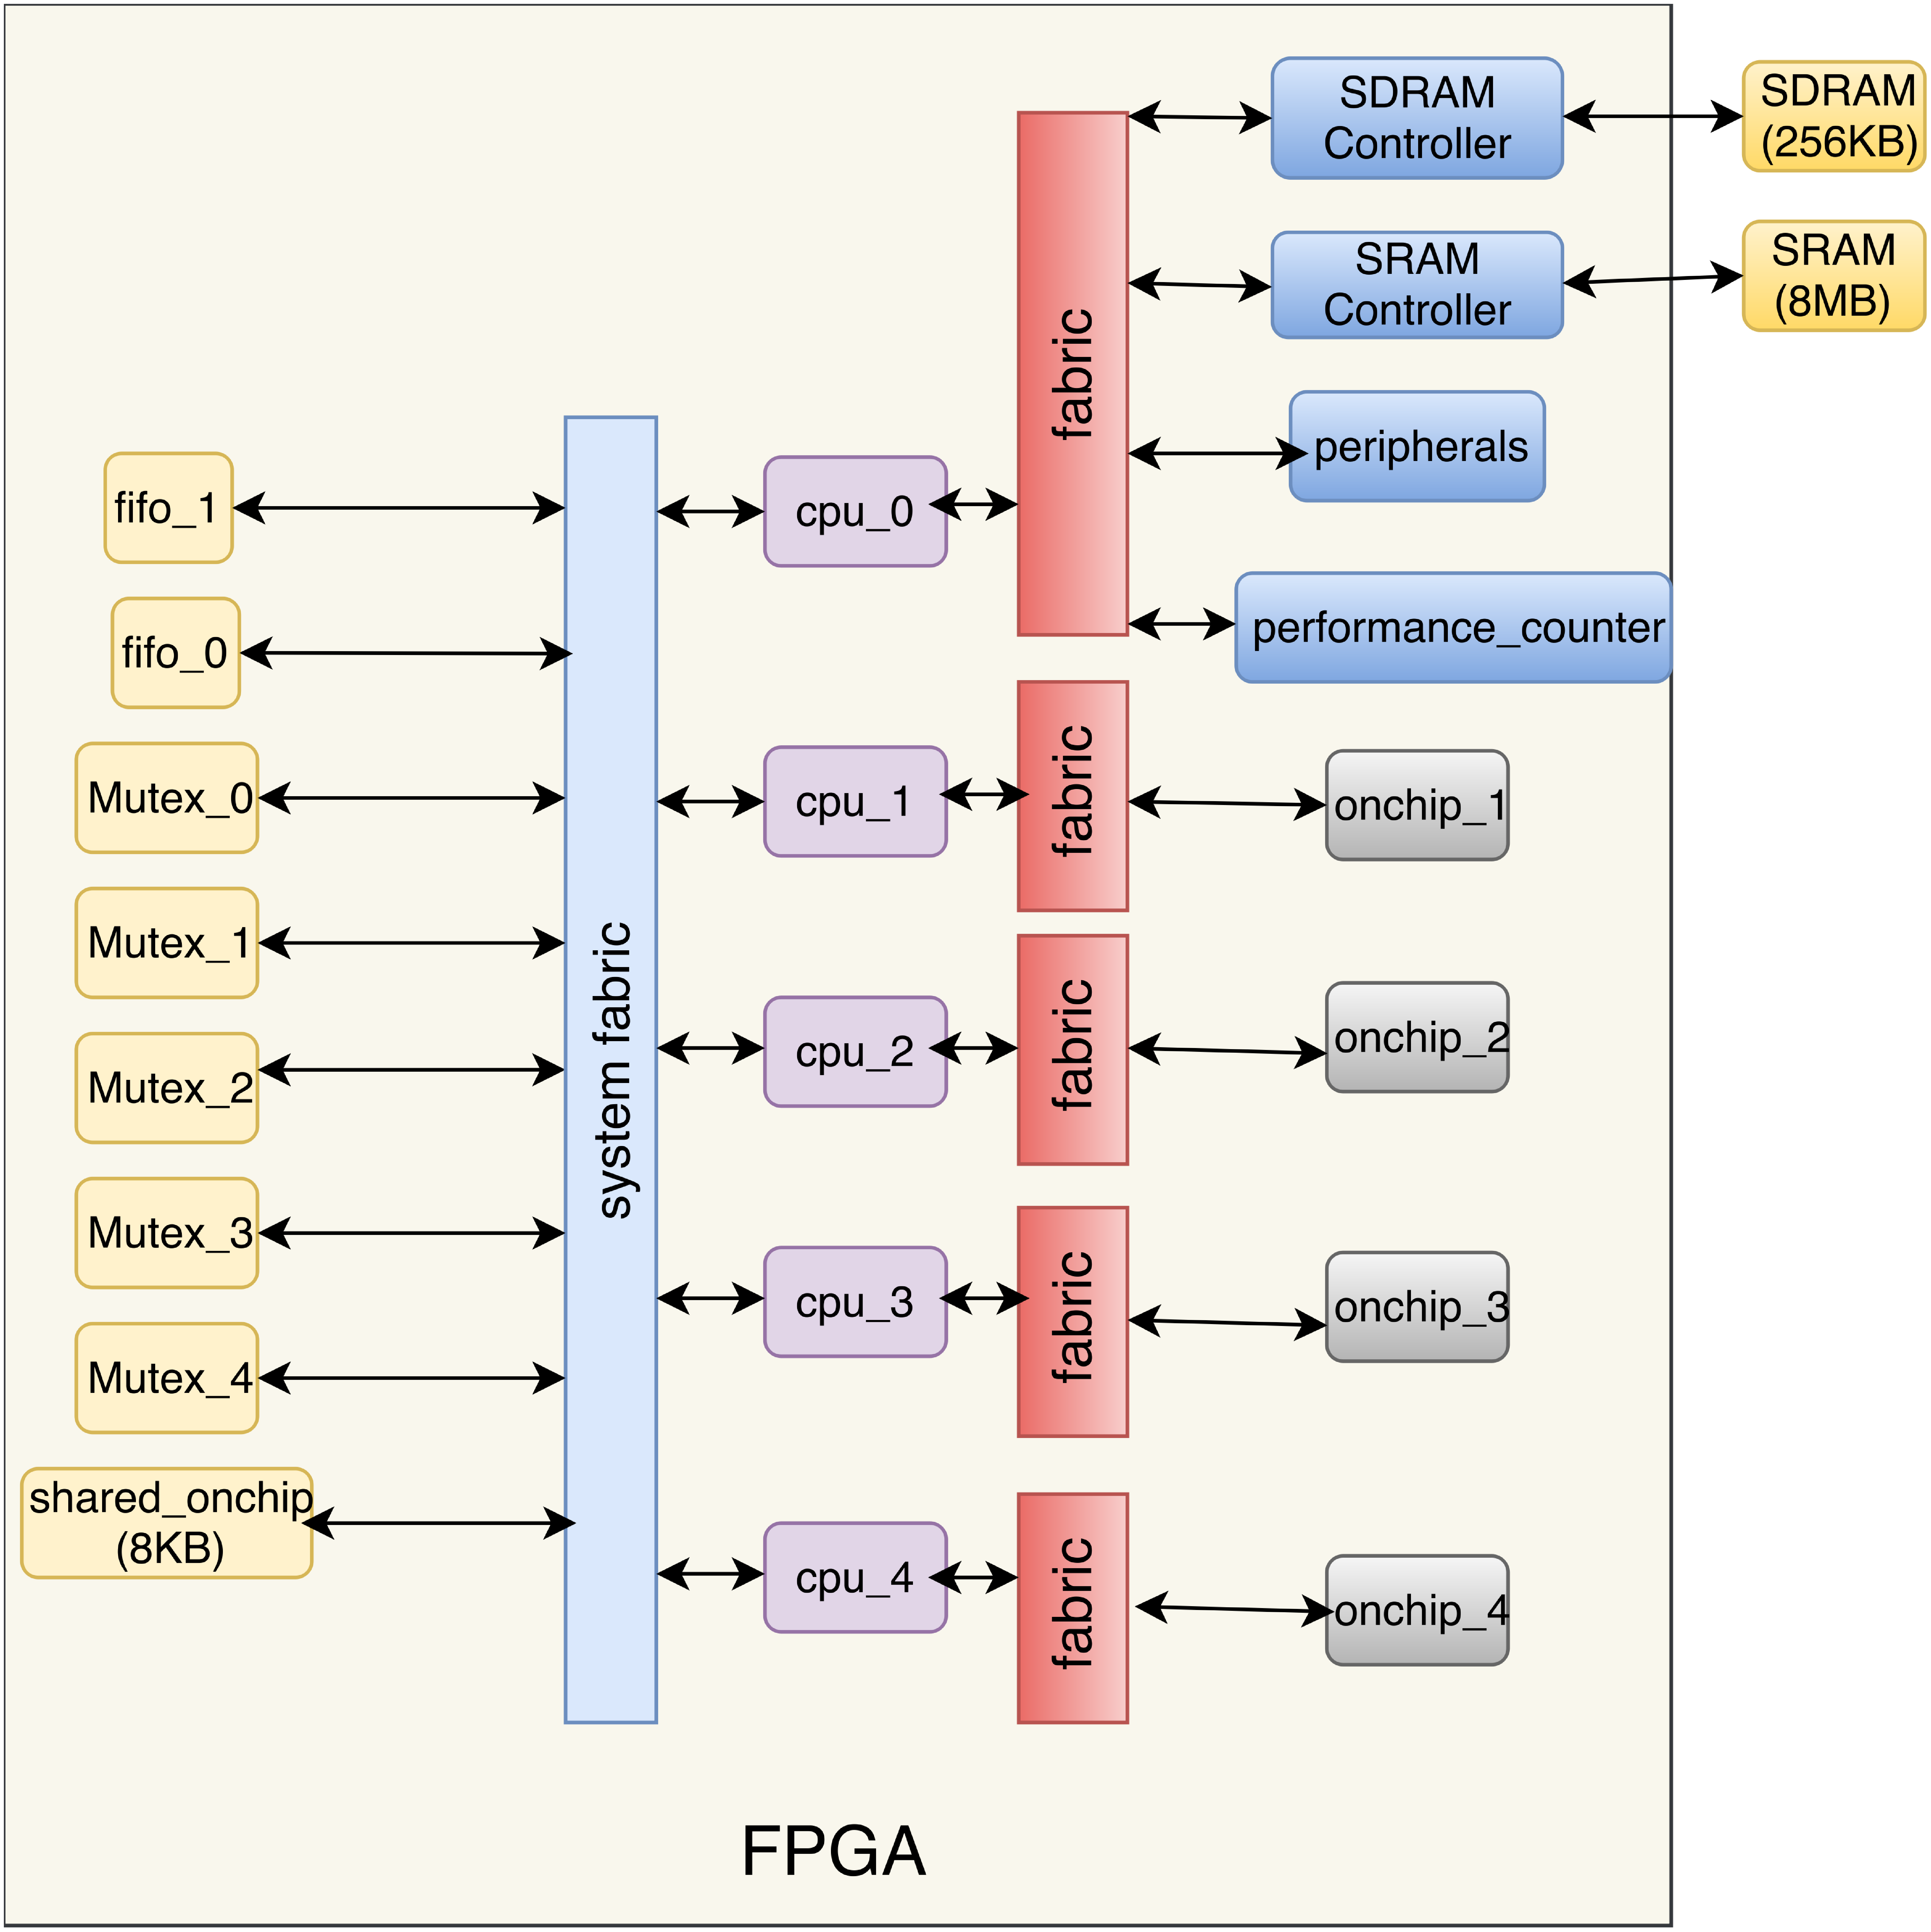
\includegraphics[width=10cm]{platform.eps}
  \caption{Platform Architecture}	
  % \label{fig_sim}
  \end{figure}
  
  %CPU\_0 is connected to SDRAM, SRAM, Timer\_0\_A, Timer\_0\_B, jtag\_uart\_0, switches, LEDs, HEX, buttons, performance counter, mutex\_0-4, fifo\_0-1 and shared\_onchip. CPU\_1, CPU\_2, CPU\_3 and CPU\_4 are connected to mutex\_0-4, fifo\_0-1 and their own onchip memory, timer and jtag\_uart.
  Through analyzing the given QSYS file and documents, we
  observed following facts: \\1.The data master is connected to
  both memory and peripheral components while the instruction
  master is only connected to memory components. \\2.The given
  architecture has five CPUs. \\3.The CPUs are connected to the
  shared on-chip memory and only CPU 0 has access to other
  peripherals such as buttons, switches. \\4.There are five mutexes
  and two fifo buffers which are shared between all CPUs.
  \subsection{Shared Resourses}
  \par The shared memory can be accessed by all the CPUs and
thus mutex logic is used to secure the communication between
shared memory and the CPUs. For example, the data in the
shared memory is accessed by any one CPU, it will lock the
mutex so that simultaneously another CPU will not be able to
access it. Other CPUs have to wait till the mutex is unlocked.
\par Mutex:The mutex core provides a protocol to ensure mutually exclusive ownership of a shared resource. The mutex
core provides a hardware-based operation allowing software
in a multiprocessor environment to determine which processor
owns the mutex. There are 5 mutex available.
\par On-Chip fifo Memory:a contiguous memory space with dedicated segments of memory allocated for 16 channels. Data
is delivered to the output interface in the same order it was
received on the input interface for a given channel.
\subsection{SRAM and peripherals}
\par SRAM/SDRAM: Only CPU 0 has access to the SDRAM
of 8MB and the SRAM of 512 KB.
\par Peripherals: Every CPU has internal peripherals and only
CPU 0 is connected to external peripherals such as buttons,
LEDs, switches and seven segment display.
\section{Functional Specification of Module}
  \subsection{Synchronous Dataflow}
  There are 5 SDF actors for processing an image: rgbToGray, resizeImg, brightness correct, sobel and toASCII.
  RgbToGray is an actor with 1 input signal and 1 output signal.
  When rgbToGray fires, it consumes $x_0 * y_1$ tokens and produces $x_1 * y_1$ tokens.
  resizeImg is a SDF with 1 input signal and 1 output signal. 
  When resizeImg fires, it consumes $x_1 * y_1$ tokens and produces $x_2 * y_2$ tokens.
  Brightness correct is a SDF with 1 input signal and 1 output signal. 
  When brightness correct fires, it consumes $x_2 * y_2$ tokens and produces $x_2 * y_2$ tokens.
  Sobel is a SDF with 1 input signal and 1 output signal. 
  When sobel fires, it consumes $x_2 * y_2$ tokens and produces $x_3 * y_3$ tokens.
  ToASCII correct is a SDF with 1 input signal and 1 out put signal. 
  When brightness correct fires, it consumes $x_3 * y_3$ tokens and produces $x_3 * y_3$ tokens.
  Then the final tokens will become the out put of the system. Hence, the system consumes $x_0 * y_1$ tokens and produces $x_3 * y_3$ tokens.
  When The SDF for image processing is shown as Figure 2.
  \begin{figure*}[h]
    \centering
    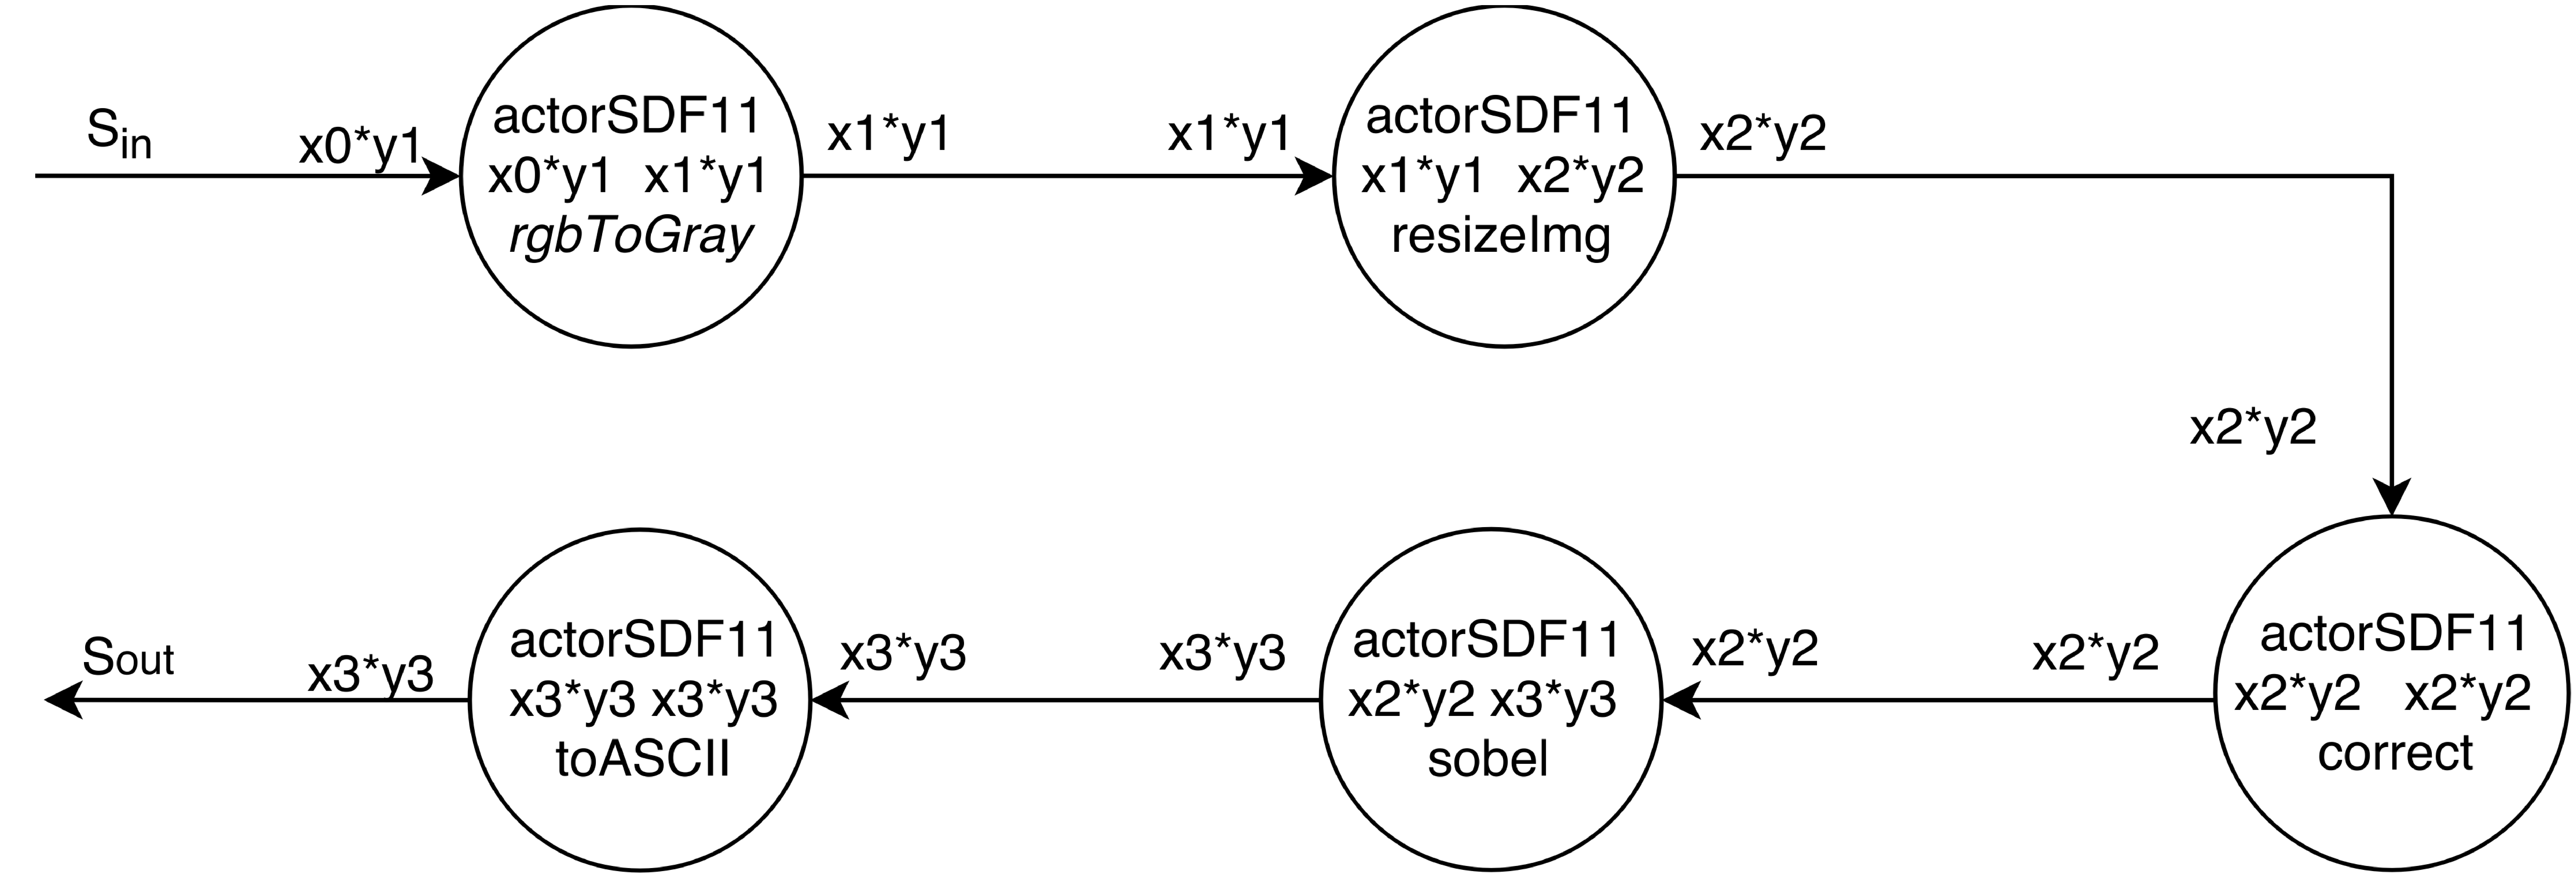
\includegraphics[width=15cm]{sdf.eps}
    \caption{Parameterized Synchronous Data Flow of Image Processing}	
    % \label{fig_sim}
    \end{figure*}
    
    \subsection{Procedures for Image Processing}
    % no \IEEEPARstart
    %\subsection{Basic Procedures}
 
  
    \textbf{Convert RGB to Gray}

    A grayscale image is one in which the value of each pixel is a single sample representing only an amount of light, that is, it carries only intensity information. Images of this sort are composed exclusively of shades of gray, varying from black at the weakest intensity to white at the strongest. And in order to get grayscale of every pixels in a typical RGB pictures, the Formula (1) is used.

  \begin{equation}
 \displaystyle Y = 0.3125 \times R + 0.5625 \times G + 0.125 \times B
  \end{equation}

  \textbf{Resize an Image}

    The next step is to resize an image. The strategy for resizing is to merge the four pixels into one pixel. As result, the total size will decrease to one fourth of the original picture. Formula for resizing is shown as Fomula 2.
    \begin{figure*}[h]
  \begin{equation}%
    \centering
    \begin{split}
    \begin{bmatrix}%
      y_{11} & y_{21} & y_{31} & y_{41} & \cdots \\
      y_{12} & y_{22} & y_{32} & y_{42} & \cdots \\
      y_{13} & y_{23} & y_{33} & y_{43} & \cdots \\
      y_{14} & y_{24} & y_{34} & y_{44} & \cdots \\
      \vdots & \vdots & \vdots & \vdots & \ddots
    \end{bmatrix}
    \qquad\mapsto\qquad
    \begin{bmatrix}
      y'_{11} = \frac{y_{11} + y_{21} + y_{12} + y_{22}}{4}
      & y'_{21} = \frac{y_{31} + y_{41} + y_{32} + y_{42}}{4}
      & \cdots \\
      y'_{12} = \frac{y_{13} + y_{23} + y_{14} + y_{24}}{4}
      & y'_{22} = \frac{y_{33} + y_{43} + y_{34} + y_{44}}{4}
      & \cdots \\
      \vdots  & \vdots  & \ddots
    \end{bmatrix}
  \end{split}
  \end{equation}
\end{figure*}
  
  
   
    \textbf{Brightness Correction}

    In order to correct the brightness level in the picture, the maximum and minimum value of the brightness need to be found out before adjustment of brightness level of the image can be done. 
    Brightness level need to be adjusted by using four threshold levels according to the maximum and minimum value of the pictures which has been detected in the former procedure.
  
    \textbf{Sobel Edge Detection}

    The Sobel operator performs a 2-D spatial gradient measurement on an image and so emphasizes regions of high spatial frequency that correspond to edges. Typically it is used to find the approximate absolute gradient magnitude at each point in an input grayscale image. Formula of Sobel operator is shown as below.
    % \begin{equation}%
    %   \vspace*{-1em} 
    
  \begin{align*}%
    &K_x=
    \begin{bmatrix}%
      -1 & 0 & 1 \\
      -2 & 0 & 2 \\
      -1 & 0 & 1
    \end{bmatrix}
    \qquad K_y=
    \begin{bmatrix}
      -1 & -2 & -1 \\
      0 & 0 & 0 \\
      1 & 2 & 1 
    \end{bmatrix}\\
    & G_x = \mathit{image} * K_x \qquad G_y = \mathit{image} * K_y \\
    & G = \sqrt{ G_x^2 + G_y^2 }
  \end{align*}

% \end{equation}
  % \caption{Sobel Operator}	
  % \label{fig_sim}
  % \end{figure}
  \textbf{Output ASCII images}
  The last step is to convert the grayscale into ASCII characters and output these characters on terminal to show the result of image processing. 
\subsection{Importance of SDF}
The SDF model consists of functions describe above, the
overall function of this SDF is to take a series of RGB
images, resize them and extract the edges, transfer every
pixel into equivalent ASCII code which represent the
brightness level. Within this program, a control progress
is implemented to detect the contrast of brightness, if the
contrast is not enough for edges detection, the image will be
corrected to fulfill the requirement.
\section{Parallel Patterns and Parallelization}
Pipelining can be applied in this application that apply a sequence of operations to
each element in a data set.Because the image processing is typical streaming application, and caculations on different pictures are independent.Therefore this application has a potential to realize pipeline parallelization. Pipeline parallelization can execute a sequence of calculations on a sequence of data elements(images). Therefore, we can assign each task to a PE and design a mechanism to forward data from one task to another.Speedup limited by number of stages and the slowest stage. If cost of sending individual elements ,communication cost,is high, aggregation is important. And on the contrary if a task consume too much time, we can spill this task into two different tasks.
 
  \section{Implementation}  
  \subsection{Bare Metal}
    For the bare-metal implementation, basic procedures are called sequentially. The sequence is rgbToGray, resizeImg, brightCorrect, sobel and at last printAscii. 
    RgbToGray will be called from main() and a pointer to images will be passed as 
    an argument. Then at the end of every basic functions, the next function will be called and the 
    pointer to the processed image will be passed on the argument.
    \subsection{RTOS}
    For RTOS implementation, we separate it to be
five tasks: grayscale function, resize function, brightness correct function, sobel function and printASCII function. Every basic function will be put on seperate tasks. Hence,
     there are 5 tasks. Tasks communicate with each other with 5 semaphores. Semaphores are used to control the execution order of tasks and access of shared on-chip memories.According to
the initial order of the application, we set the semaphore of
task RgbToGray to 1 initially, and successively pend its own
semaphore and post the semaphore of the subsequent task to
continue processing.RTOS implementation can be shown as Figure 3.
   
     \begin{figure}[h]
      \centering
      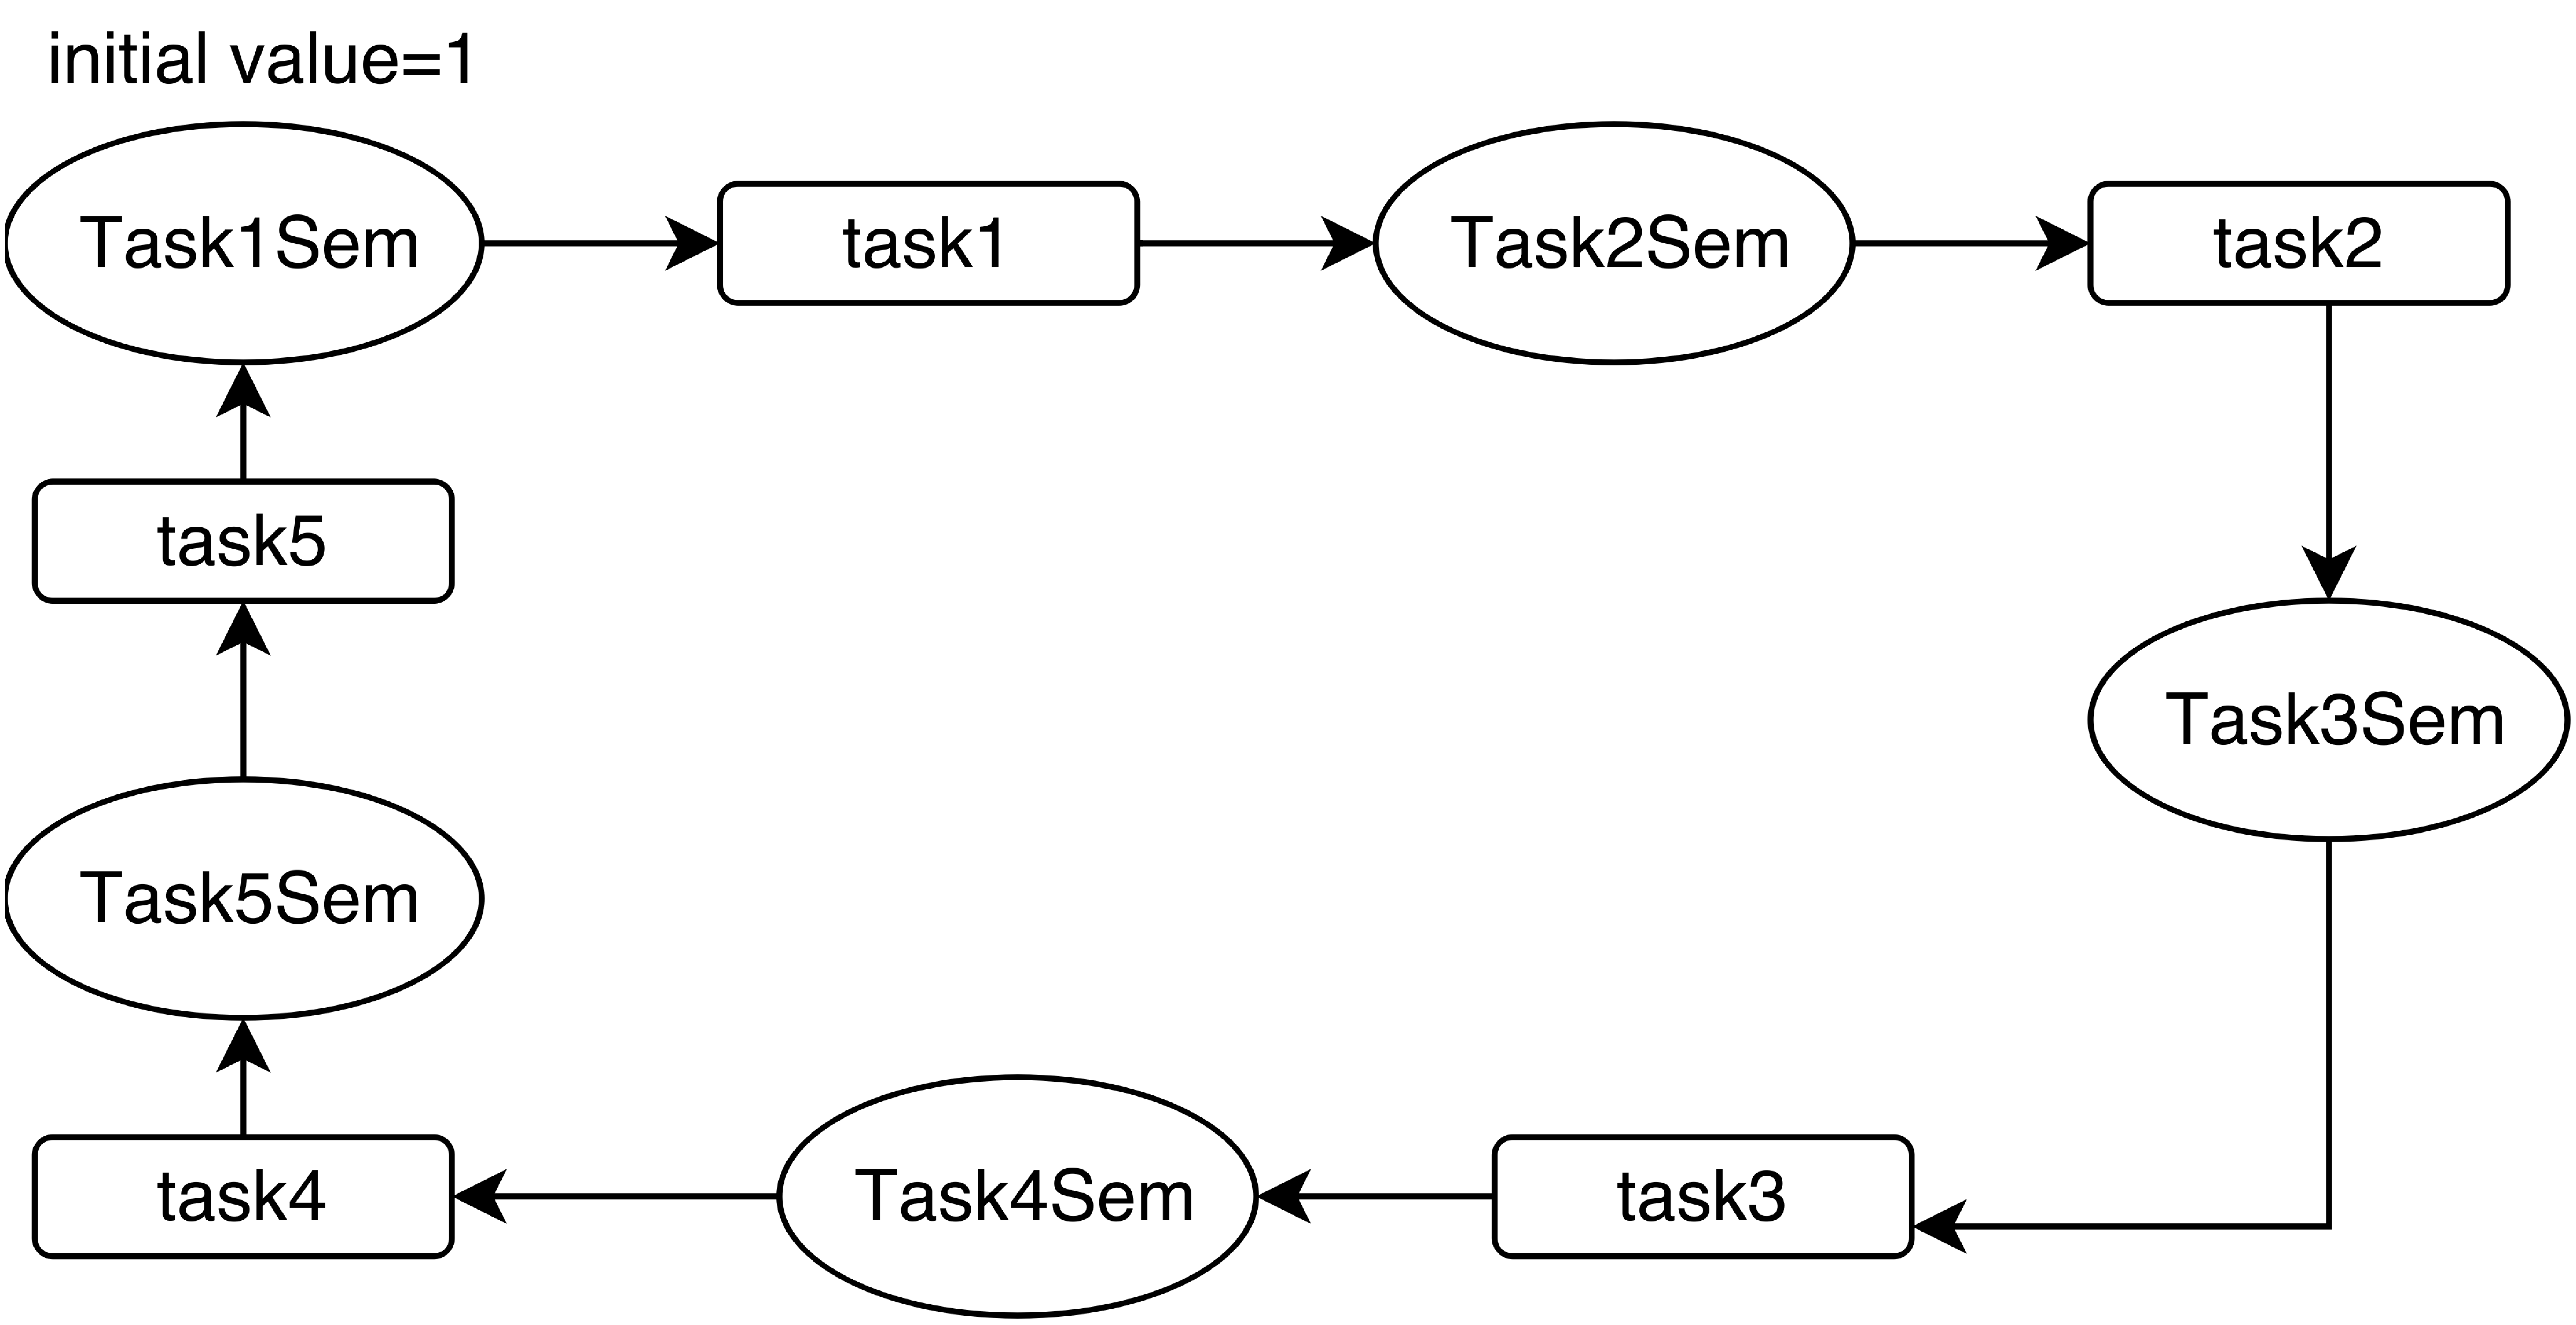
\includegraphics[width=8cm]{Semaphore.eps}
      \caption{RTOS Implementation}	
      % \label{fig_sim}
      \end{figure}
      \subsection{Multi-core}
      Multi-core application also has five parts like single core, and we implement grayscale function and store the ASCII back to the SRAM in CPU0, because only the CPU0 can get access to the SRAM, so it can get the RGB image from SRAM and store ASCII back to the SRAM. We also implement resize function and brightness correct function in CPU1, sobel function function in CPU2, and printASCII function in CPU3. On flow chart below, we show how it works. 
      \begin{figure}[h]
        \centering
        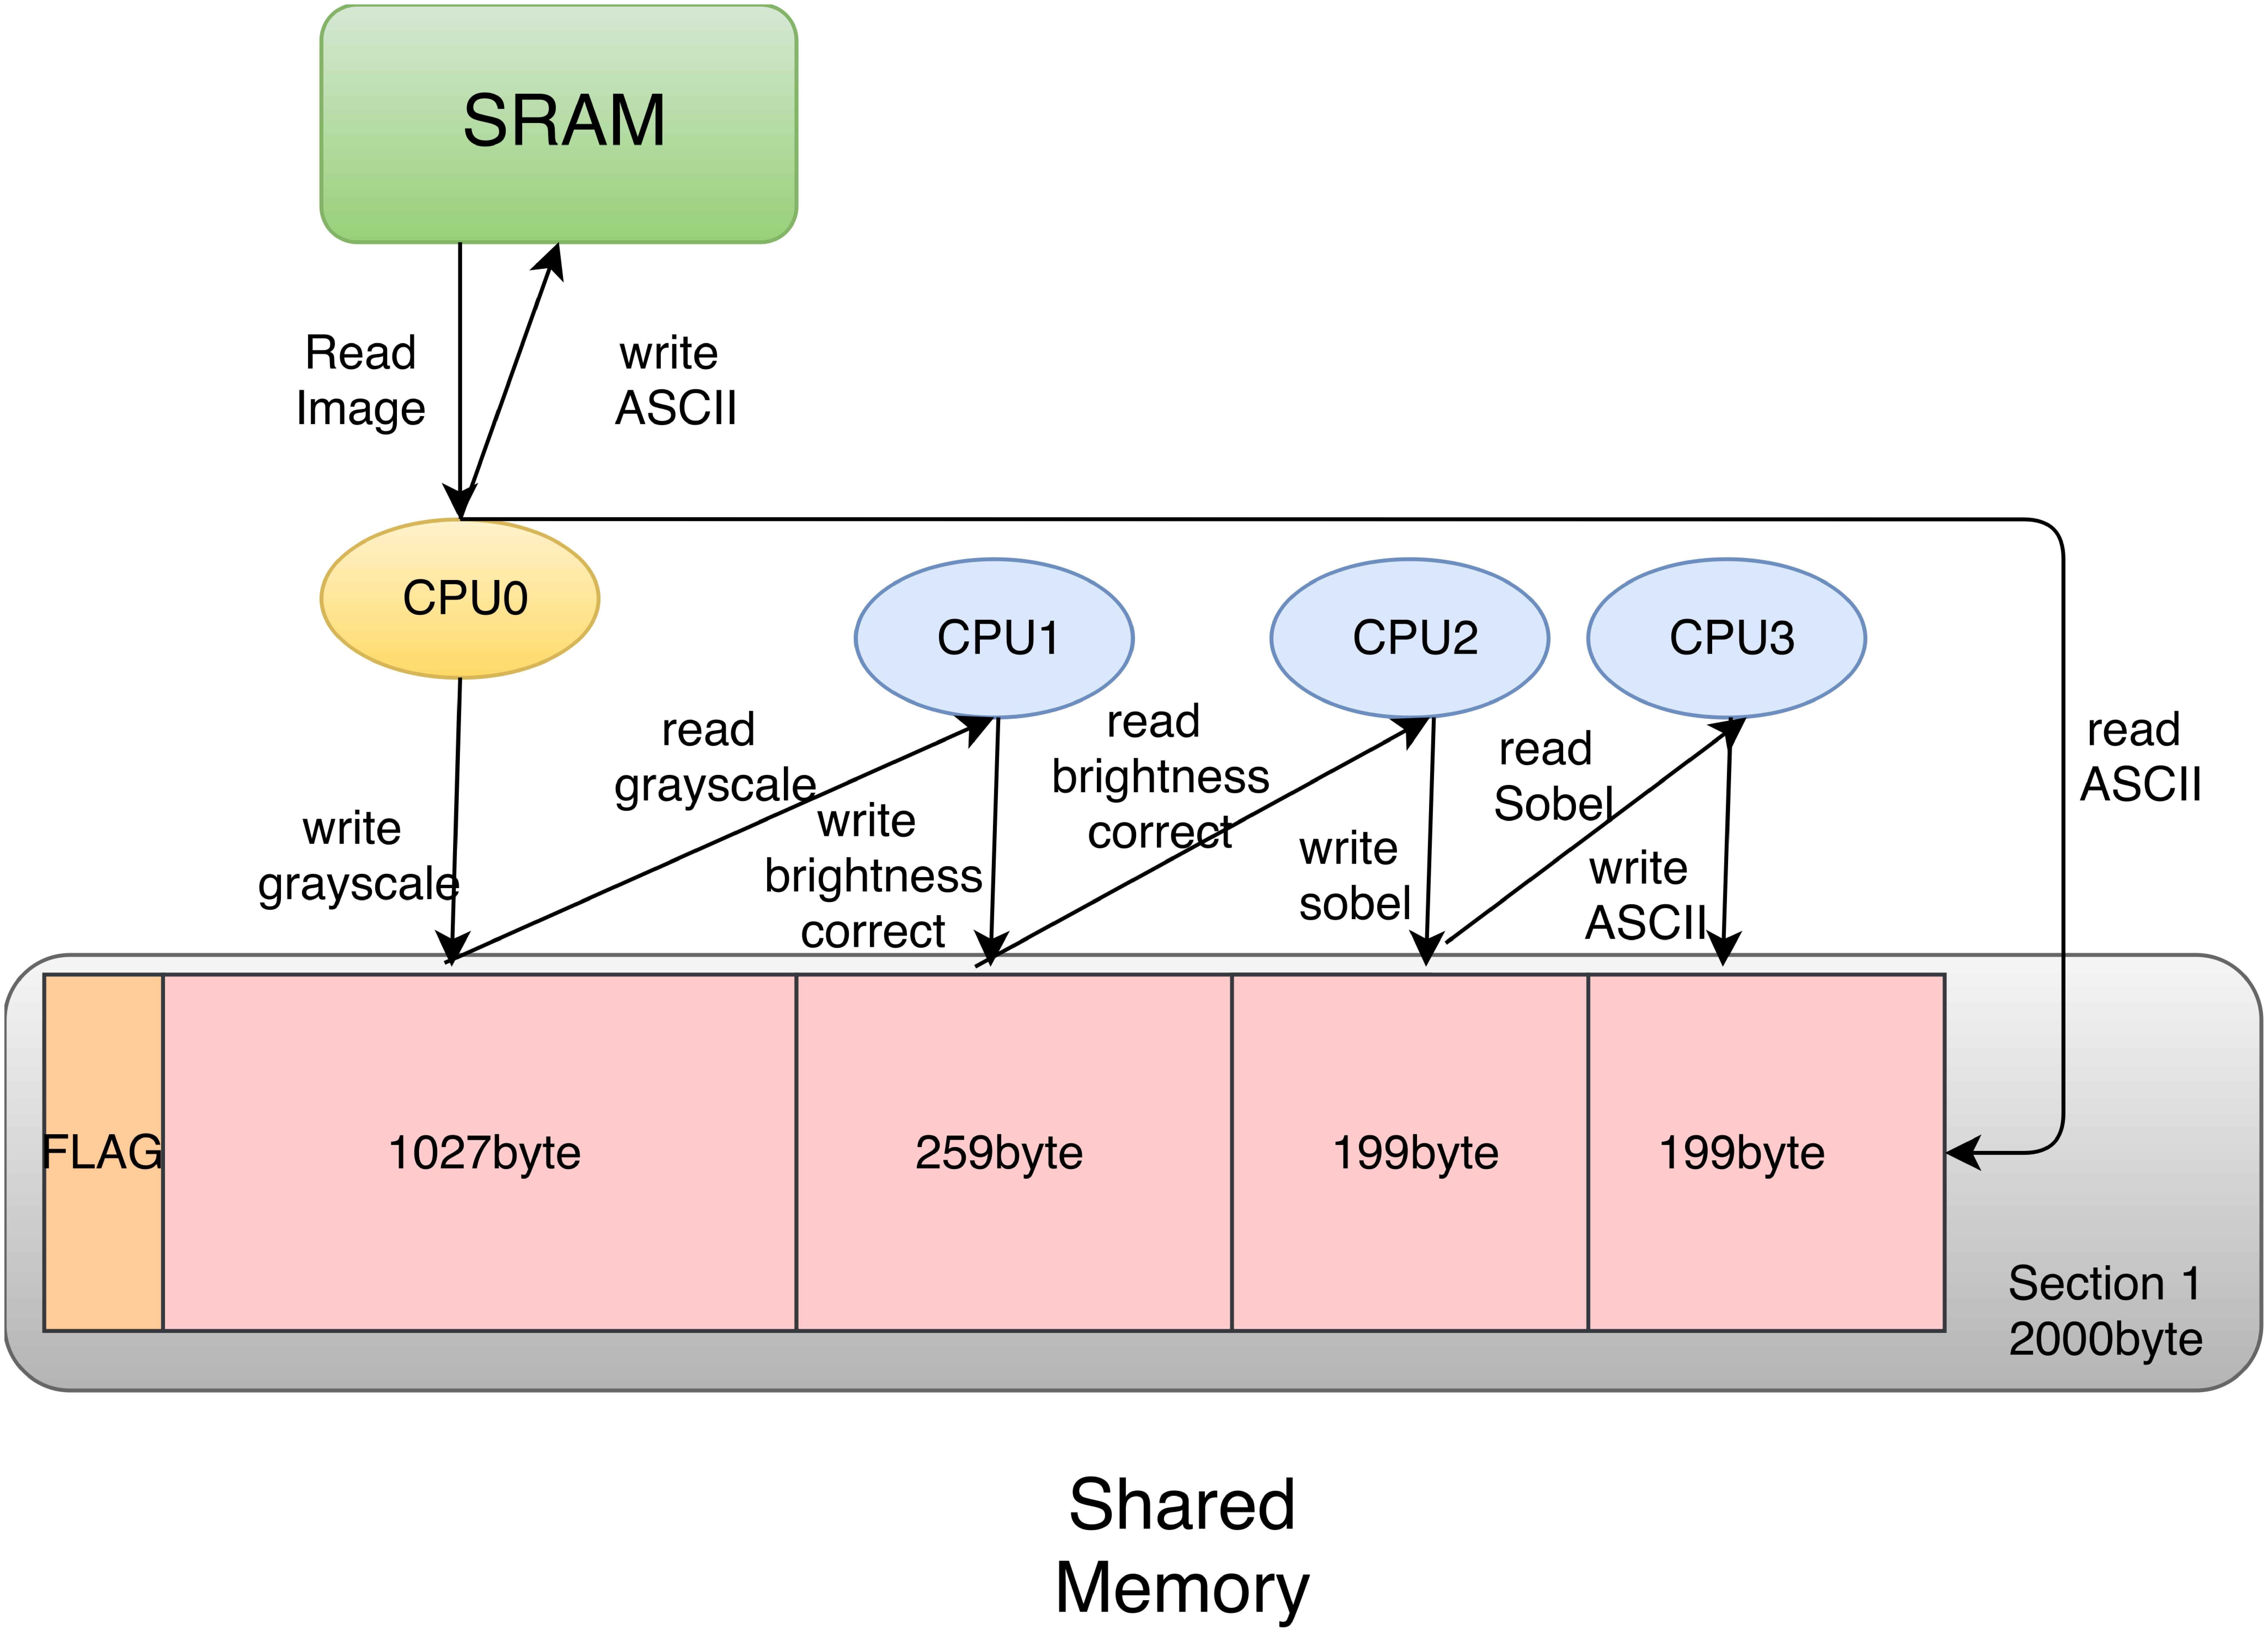
\includegraphics[width=9cm]{multimodel.eps}
        \caption{Mapping Plan}	
        % \label{fig_sim}
        \end{figure}
      \par We divide the shared memory into four independent sections and each section is responsible for one picture. The size of each section is fixed and it is 2048 byte.So we can store the grayscale dataset at the beginning of each section and it will occupy $32*32+3=1027$ byte of the shared memory space, since the first three byte always store the size of X, the size of Y and the maximum value of the grayscale. It is followed by image dataset after resize and brightness correct function and it will take up $16*16+3=259$ byte of of the shared memory space. The next part is dataset after sobel function and it accounts for $14*14+3=199$ byte of the shared memory space. The last part of each section is ASCII storage and it contains the same shared memory space as the dataset processed by sobel function. Therefore, in total the size of each section which is being used is $1027+259+199+199=1684$ byte which is less than 2048 allocated for each section. 
      \par And Apart from these four sections, there is also a one-byte flag used to store the current state of the process. The flag contains eight binary bit, every two of them forms a counter which can calculate the number of image being disposed. 00 stands for the smallest number zero and 11 stands for the largest number three. And the first two bits represents the counter relating to grayscale function. The remaining six bits represents brightness correctness counter, sobel counter and printASCII counter respectively. The schedule of multi-cores implementation is showed below.
      \begin{figure}[h]
        \centering
        \includegraphics[width=9cm]{schedule.eps}
        \caption{Multi-core Schedule}	
        % \label{fig_sim}
        \end{figure}
  
    
    % An example of a floating figure using the graphicx package.
    % Note that \label must occur AFTER (or within) \caption.
    % For figures, \caption should occur after the \includegraphics.
    % Note that IEEEtran v1.7 and later has special internal code that
    % is designed to preserve the operation of \label within \caption
    % even when the captionsoff option is in effect. However, because
    % of issues like this, it may be the safest practice to put all your
    % \label just after \caption rather than within \caption{}.
    %
    % Reminder: the "draftcls" or "draftclsnofoot", not "draft", class
    % option should be used if it is desired that the figures are to be
    % displayed while in draft mode.
    %
    %\begin{figure}[!t]
    %\centering
    %\includegraphics[width=2.5in]{myfigure}
    % where an .eps filename suffix will be assumed under latex, 
    % and a .pdf suffix will be assumed for pdflatex; or what has been declared
    % via \DeclareGraphicsExtensions.
    %\caption{Simulation results for the network.}
    %\label{fig_sim}
    %\end{figure}
    
    % Note that the IEEE typically puts floats only at the top, even when this
    % results in a large percentage of a column being occupied by floats.
    
    
    % An example of a double column floating figure using two subfigures.
    % (The subfig.sty package must be loaded for this to work.)
    % The subfigure \label commands are set within each subfloat command,
    % and the \label for the overall figure must come after \caption.
    % \hfil is used as a separator to get equal spacing.
    % Watch out that the combined width of all the subfigures on a 
    % line do not exceed the text width or a line break will occur.
    %
    %\begin{figure*}[!t]
    %\centering
    %\subfloat[Case I]{\includegraphics[width=2.5in]{box}%
    %\label{fig_first_case}}
    %\hfil 
    %\subfloat[Case II]{\includegraphics[width=2.5in]{box}%
    %\label{fig_second_case}}
    %\caption{Simulation results for the network.}
    %\label{fig_sim}
    %\end{figure*}
    %
    % Note that often IEEE papers with subfigures do not employ subfigure
    % captions (using the optional argument to \subfloat[]), but instead will
    % reference/describe all of them (a), (b), etc., within the main caption.
    % Be aware that for subfig.sty to generate the (a), (b), etc., subfigure
    % labels, the optional argument to \subfloat must be present. If a
    % subcaption is not desired, just leave its contents blank,
    % e.g., \subfloat[].
    
    
    % An example of a floating table. Note that, for IEEE style tables, the
    % \caption command should come BEFORE the table and, given that table
    % captions serve much like titles, are usually capitalized except for words
    % such as a, an, and, as, at, but, by, for, in, nor, of, on, or, the, to
    % and up, which are usually not capitalized unless they are the first or
    % last word of the caption. Table text will default to \footnotesize as
    % the IEEE normally uses this smaller font for tables.
    % The \label must come after \caption as always.
    %
    %\begin{table}[!t]
    %% increase table row spacing, adjust to taste
    %\renewcommand{\arraystretch}{1.3}
    % if using array.sty, it might be a good idea to tweak the value of
    % \extrarowheight as needed to properly center the text within the cells
    %\caption{An Example of a Table}
    %\label{table_example}
    %\centering
    %% Some packages, such as MDW tools, offer better commands for making tables
    %% than the plain LaTeX2e tabular which is used here.
    %\begin{tabular}{|c||c|}
    %\hline
    %One & Two\\
    %\hline
    %Three & Four\\
    %\hline
    %\end{tabular}
    %\end{table}
    
    
    % Note that the IEEE does not put floats in the very first column
    % - or typically anywhere on the first page for that matter. Also,
    % in-text middle ("here") positioning is typically not used, but it
    % is allowed and encouraged for Computer Society conferences (but
    % not Computer Society journals). Most IEEE journals/conferences use
    % top floats exclusively. 
    % Note that, LaTeX2e, unlike IEEE journals/conferences, places
    % footnotes above bottom floats. This can be corrected via the
    % \fnbelowfloat command of the stfloats package.
    
    
    
    
    
  \section{Performance Optimization}
  First, We optimize sobel operator, when it comes to square root, we did not use $G = \sqrt{ G_x^2 + G_y^2 } $, we use $G = |G_x| + |G_y| $ instead. Because square root function can consume a large amount of time, we use absolute values to do the approximation. This approximation is correct because in this project, 
  this approximation results to an maximum error of 74.68 on grayscale values when $ |G_x| = |G_y| = 127.5$. In this case, the approximation result for $G$ is $255$ while it should be $180.31$ using square roots. Before sobel optimization, the soble function accounts for nearly half of the total execution time. And it just takes up 17 percent of the total execution time after optimization. It is much faster to compute and thus optimize the performance.
  \par Second, when converting RGB picture to greyscale, we use the approximation of  use binary shift instead of multiplication and division. Because multiplication and division cost 3 times more time than binary shift. For example, if we use multiplication and division to calculate the equation of, it should be like this $G = (5*R + 9*G + 2*B)/16 $, and the performance of that is 30 pictures per second. However, if authors use binary shift like this,$G = (R>>2) + (R>>4) + (G>>1) + (G>>4) + (B>>3) $
  , and the performance will increase significantly, 180 pictures per second. So we need to avoid multiplication and division as much as possible and use binary shift function instead. 
  \par Third, we hoist the common statement from the loop to avoid repeat computation of the similar statement in the loop. 

  Fouth, we use int array to store char values that are on shared onchip memory to SRAM.
  For example, in this project, a char is 1 byte and an int is 4 bytes, which means reading or writing one
  integers are equivalent to reading or writing 4 chars. This can reduce the number of reading or writing, thereby increasing the 
  Throughput.


  % conference papers do not normally have an appendix
  
  % \begin{align}
  \section{Measurement and Analysis}
  The project is conducted on DE2 board. There are three implementations: single core without RTOS, single core with RTOS and multi-core. The performance and memory footprint of these three implementation are measured. 
  % \pagebreak[4]
  \subsection{Single Core}
  Throughputs and footprints of two implementation are shown in Table 1. Performance counter reports are shown in Table 2 and Table 3, where Table 2 is table for bare metal implementation and Table 3 is table for RTOS implementation. The total percentage does not equal to 100 percent, because some time is spent on context switch. The result suggests that for single core, RTOS implementation is less efficient than bare metal. It is because RTOS has too many overheads for running tasks, which slows down the speed.  
  % \begin{center}
  \begin{table}
  \centering
  \caption{Single Core Measurements}
  \begin{tabular}[t]{  ccc } 
  \hline
  \centering
  & Single Core (RTOS)& Single Core (Bare Metal)\\
  \hline
  Throughput[s-1]& 106 & 112 \\
  SRAM(Byte)& 157244 & 106820 \\
  \hline
  \end{tabular}
  % \end{center}
  \end{table}
  
  \begin{table}[h]
  \centering
  \caption{Bare Metal Performance}
  \begin{tabular}[t]{  ccccc  } 
  \hline
  Section & \% & Time (sec) & Time (clock)& Occurrences \\
  \hline
  rgbToGray & 30.7 & 0.00273 & 136490 & 1\\
  resizeImg& 10.7 & 0.00095 & 47600 & 1\\
  brightCorrect& 6.31 & 0.00056 & 28028 & 1\\
  sobel& 23.6 & 0.00210 & 104858 & 1\\
  printAscii& 28.3 & 0.00252 & 125820 & 1\\
  \hline
  Total time & 100 & 0.00888 & 444171 & 1\\ 
  \hline
  \end{tabular}
  % \end{center}
  \end{table}
  
  \begin{table}[h]
  \centering
  \caption{RTOS Performance}
  \begin{tabular}[t]{  ccccc } 
  \hline
  Section & \% & Time (sec) & Time (clock)& Occurrences \\
  \hline
  rgbToGray & 30.2 & 0.00283 & 141605 & 1\\
  resizeImg& 10.5 & 0.00099 & 49350 & 1\\
  brightCorrect& 3.52 & 0.00033 & 16501 & 1\\
  sobel& 24.9 & 0.00233 & 116642 & 1\\
  printAscii& 27.7 & 0.00260 & 129792 & 1\\
  \hline
  Total time & 100 & 0.00937 &468572 & 1 \\
  \hline
  \end{tabular}
  % \end{center}
  \end{table}
  
  \subsection{Multi-core}
  Throughputs and footprints of two implementation are shown in Table 4. Both throughput and footprints meets the design constraints which are 
  320 or higher throughput and 45KB or less footprints.
  % \begin{center}
  \begin{table}[h]
  \centering
  \caption{Multi-Core Measurements}
  \begin{tabularx}{8.5cm}{ c m{1cm}<{\centering} m{1cm}<{\centering} m{1cm}<{\centering} } 
  \hline
  &Single Core (RTOS)&Single Core (Bare Metal)& Multi-processor\\
  \hline
  Throughput[s-1] &106 &112& 323 \\
  SRAM[Byte]&157244 &106820 &23772 \\
  OnChip CPU 1 [bytes]&--&--&3244\\
  OnChip CPU 2 [bytes]&--&--&3100\\
  OnChip CPU 3 [bytes]&--&--&2096\\
  OnChip CPU 4 [bytes]&--&--&1856\\
  OnChip Shared [bytes]&1027&0&6737\\
  Total Memory [bytes]&157244&106820&40805\\
  \hline
  \end{tabularx}
  \end{table}
% \end{align}
  % \end{center}
  \subsection{Evaluations}
  The multi-core implementation has the highest throughput which is almost three times the figure of single core implementations. In theory,
  the throughput of multi-core implementation can be 5 times that of single core implementations. But because of our mapping, calculations are not distributed equally to every core. The throughput 
  of multi-core implementation is decided by cpu\_0 which is mapped to finish the convertion of rgb to grayscale because it takes longest time.

  Single core implementations can easily ensure the sequence of executing procedures. For bare metal implementaion, because C language is a imperative
  language, which means functions will be executed sequentially. For RTOS implementation, some tools can be used, for example semaphores, to communicate 
  between tasks, thereby ensuring the sequence of execution. When it comes to multi-core, CPUs have to communicate via shared memory. Techniques such as flags and fifos should be use 
  to ensure a correct output, which means there will be overheads for communications that can slow down the execution speed. There are also problems when 
  communicating via shared memory, the data corruption. Data on shared memory can be changed by more than one processor. If the programme is not 
  well written, there will be incorrect results.

  For resource consumption, bare metal implementation consumes least because it has only one core and use less memory. RTOS implementation use more resources than 
  bare metal implementation because it needs time for communication between tasks and more overheads for OS. The multi-core implementation consumes 
  most resources because it uses 4 cores and 4 memory sections with only 3 times the throughput of single core implementations. Therefore, for economical consideration,
   we should choose bare metal implementation.
\section{conclusion}
\par In conclusion, compared with single core implementation, multi-core implementation can achieve much better throughput. But in the mean time, it requires more footprint and hardware resourses. Therefore we have to consider this trade-off option when implementing image processing algorithm into the hardware architecture. 
\begin{thebibliography}{1}

\bibitem{IEEEhowto:kopka}
Kent Orthner, \emph{Applying the Benefts of Network on
a Chip Architecture to FPGA System
Design}.\hskip 1em plus
  0.5em minus 0.4em\relax Intel.

\end{thebibliography}
    % use section* for acknowledgment
    \ifCLASSOPTIONcompsoc
      % The Computer Society usually uses the plural form
      \section*{Personal Contributions}
    \else
      % regular IEEE prefers the singular form

      \section*{Personal Contributions}
    \fi
    \textbf{Jiaqi Li}\\
    Implement brightness correction and sobel functions.\\
    Conduct and debug RTOS implementation.\\
    Write contents of Procedures for Image Processing and Measurement and Analysis for the report.\\
    Use latex to format the report.\\
    Optimize the multi-core implementation to meet design constrains.


    \textbf{Guanghao Guo}\\
   Implement grayscale, resize and printAscii functions.\\
   Conduct and debug bare-metal implementation.\\
   Write contents of Hardware Architecture, Concurrent Processes Networks for the report.\\
   Draw graphs for the report.
   Transplant single core codes to the multi-core implementation
    
    
    
    
    
    % trigger a \newpage just before the given reference
    % number - used to balance the columns on the last page
    % adjust value as needed - may need to be readjusted if
    % the document is modified later
    %\IEEEtriggeratref{8}
  % * <jol.lijiaqi@gmail.com> 2018-02-04T21:44:32.447Z:
  %
  % ^.
    % The "triggered" command can be changed if desired:
    %\IEEEtriggercmd{\enlargethispage{-5in}}
    
    % references section
    
    % can use a bibliography generated by BibTeX as a .bbl file
    % BibTeX documentation can be easily obtained at:
    % http://mirror.ctan.org/biblio/bibtex/contrib/doc/
    % The IEEEtran BibTeX style support page is at:
    % http://www.michaelshell.org/tex/ieeetran/bibtex/
    %\bibliographystyle{IEEEtran}
    % argument is your BibTeX string definitions and bibliography database(s)
    %\bibliography{IEEEabrv,../bib/paper}
    %
    % <OR> manually copy in the resultant .bbl file
    % set second argument of \begin to the number of references
    % (used to reserve space for the reference number labels box)
  %   \begin{thebibliography}{1}
    
  %   \bibitem{IEEEhowto:kopka}
  %   H.~Kopka and P.~W. Daly, \emph{A Guide to \LaTeX}, 3rd~ed.\hskip 1em plus
  %     0.5em minus 0.4em\relax Harlow, England: Addison-Wesley, 1999.
    
  %   \end{thebibliography}
    
    
    
    
    % that's all folks
    \end{document}
    
    
    